% ****************************************************************************************
%              Title
% ****************************************************************************************

\frenchspacing
\raggedbottom

\pagenumbering{roman}
\pagestyle{plain}

% *******************************************************
% Titlepage
% *******************************************************
\title{\myTitle}
\begin{titlepage}
  % \pdfbookmark[1]{\myTitle}{titlepage}
  % if you want the titlepage to be centered, uncomment and fine-tune the line below (KOMA classes environment)
  %\begin{addmargin}[-1cm]{-3cm}
    \begin{center}
      \large

      \hfill

      \vfill

      \begingroup
      \color{CTtitle}\spacedallcaps{\myTitle}\\

      \vspace{5mm}

      \Large{\mySubtitle}
      \endgroup
      \medskip

      \vspace{3cm}
      A thesis proposal by\\
      \spacedlowsmallcaps{\myName} \\

      \vfill

      \myUni\\
      \myDepartment\\
      \myLocation\\
      \myTime\\
      \medskip
    \end{center}
  %\end{addmargin}
\end{titlepage}

\thispagestyle{empty}


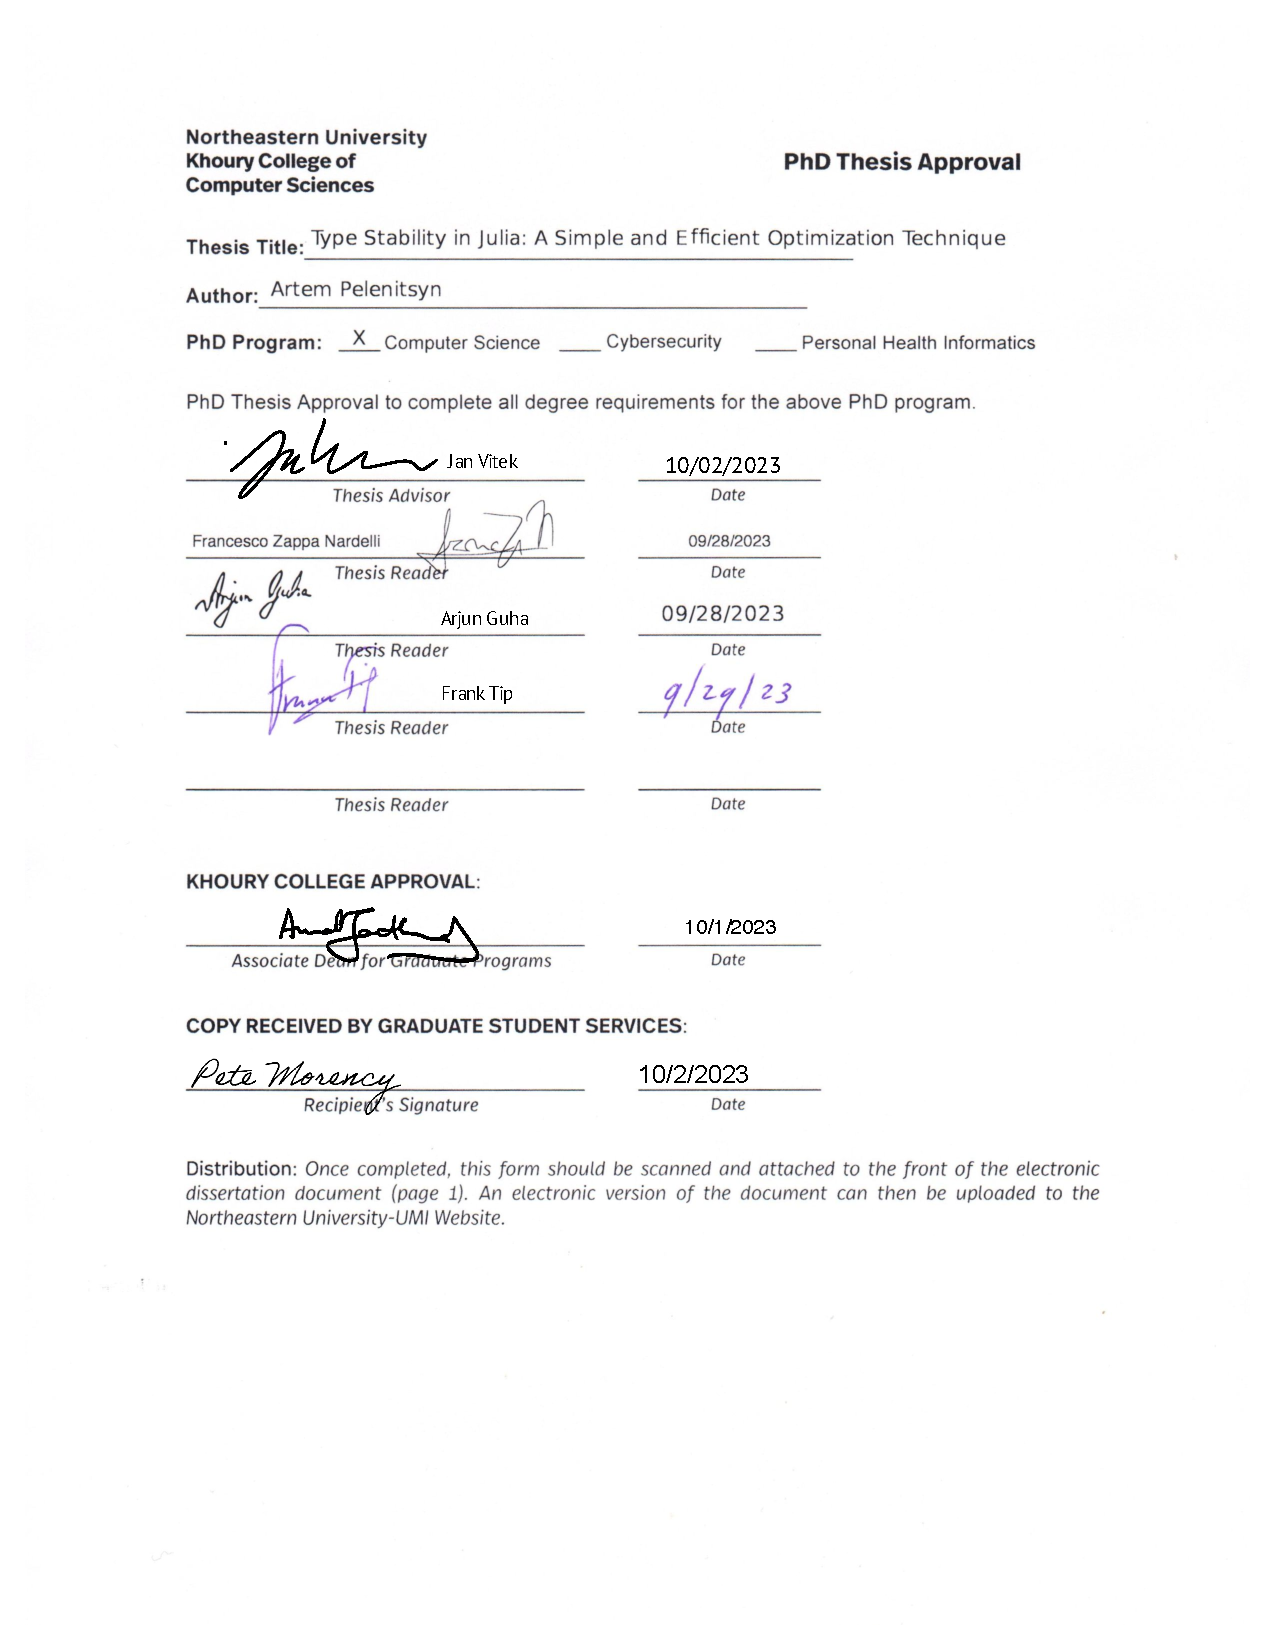
\includepdf[pages={1},noautoscale]{approval.pdf}

\chapter*{abstract}
The design space for just-in-time (JIT) compilers is big, and Julia represents one viewpoint.
The outstanding features of this viewpoint is simplicity and efficiency, which
are enabled by a clever co-design of the language and its implementation.
The combination of simplicity and efficiency also allows users to employ
language strengths and avoid common pitfalls that threaten the wide family of JIT
compilers.

My work has been focused on type stability in Julia---a program property
enabling key optimizations in the compiler.
Informally, a function is type stable if the type of
the output depends only on the types of the inputs, not their values.
In this dissertation, I make the following contributions
related to type stability.
First, an analysis of how widespread the
property is in publicly available Julia code, and what features may be related
to the property.
Second, a formal model of a JIT compiler recognizing the
property at run time and performing optimizations accordingly. Third,
an automated approach to approximate type stability without
running the program.
% Based on this approach, I wish to allow programmers expressing
% the assumptions about type stability directly in the code.

%*******************************************************
% Table of Contents (uncomment \tableofcontents)
%*******************************************************
\pagestyle{scrheadings}
% \pdfbookmark[1]{\contentsname}{tableofcontents}
\setcounter{tocdepth}{2} % <-- 2 includes up to subsections in the ToC
\setcounter{secnumdepth}{3} % <-- 3 numbers up to subsubsections
\cleardoublepage%
\phantomsection%
\addcontentsline{toc}{chapter}{Contents}
\tableofcontents

\cleardoublepage%
\phantomsection%
\addcontentsline{toc}{chapter}{\listfigurename}
\listoffigures

\cleardoublepage%
\phantomsection%
\addcontentsline{toc}{chapter}{\listtablename}
\listoftables

%********************************************************************
% Mainmatter
%*******************************************************
\cleardoublepage%
\pagestyle{scrheadings}
\pagenumbering{arabic}
%\setcounter{page}{90}
% use \cleardoublepage here to avoid problems with pdfbookmark
